\section{Deviations from the pre-analysis plan}\label{app:deviations}

\emph{A1 (before the full run).} The pilot showed that unusable replies were arithmetic errors, not refusals; under the original 95--105 rule five of the twelve models would have been excluded, removing both fine-tune pairs. Replies still outside 95--105 after one retry are therefore renormalised, and the original rule is reported as a robustness check (it excludes \nOrigRuleExcluded{} models). The temperature-0.7 check uses two seeds instead of three to stay within the GPU budget. \emph{Post hoc.} The dispersion-adjusted specification in Table~\ref{tab:robust} was added after the primary results were seen and is labelled as such.

\section{Models and failure rates}\label{app:models}

Table~\ref{tab:models} lists the models with their throughput on one RTX 4070 Ti and their reply status in the primary run; Fig.~\ref{fig:rates} breaks the status down by model and prompt language.

\begin{table}[htbp]
\caption{Models, throughput on one RTX 4070 Ti (generated tokens per second) and reply status in the primary run (240 greedy prompts per model).}
\label{tab:models}
\centering\footnotesize\setlength{\tabcolsep}{3pt}
% generated by src/viz/paper_tex.py
\begin{tabular}{@{}lllrlrrr@{}}
\toprule
Model & Developer & Origin & Params (B) & Quant. & tok/s & Refusal (\%) & Parse fail (\%) \\
\midrule
Qwen3-8B & Alibaba & China & 8.2 & Q4\_K\_M & 81 & 0.0 & 0.0 \\
Qwen2.5-7B & Alibaba & China & 7.6 & Q4\_K\_M & 91 & 0.0 & 0.0 \\
GLM-4-9B & Zhipu AI / Tsinghua & China & 9.4 & Q4\_0 & 80 & 0.0 & 0.0 \\
Llama-3.1-8B & Meta & US & 8.0 & Q4\_K\_M & 86 & 0.0 & 0.0 \\
Gemma-3-12B & Google & US & 12.2 & Q4\_K\_M & 52 & 0.0 & 0.0 \\
Phi-4-14B & Microsoft & US & 14.7 & Q4\_K\_M & 49 & 0.0 & 0.8 \\
Mistral-7B & Mistral AI & Europe & 7.2 & Q4\_K\_M & 94 & 0.0 & 0.0 \\
Mistral-NeMo-12B & Mistral AI with NVIDIA & Europe & 12.2 & Q4\_0 & 63 & 0.0 & 0.0 \\
EuroLLM-9B & UTTER consortium & Europe & 9.2 & Q4\_K\_M & 77 & 0.4 & 0.0 \\
Typhoon2-8B & SCB 10X & Thailand & 8.0 & Q4\_K\_M & 86 & 0.0 & 0.0 \\
OpenThaiGPT-1.5-7B & OpenThaiGPT & Thailand & 7.6 & Q4\_K\_M & 91 & 0.0 & 0.0 \\
EXAONE-3.5-7.8B & LG AI Research & Korea & 7.8 & Q4\_K\_M & 89 & 0.0 & 0.4 \\
\bottomrule
\end{tabular}

\end{table}

\begin{figure}[htbp]
\centering
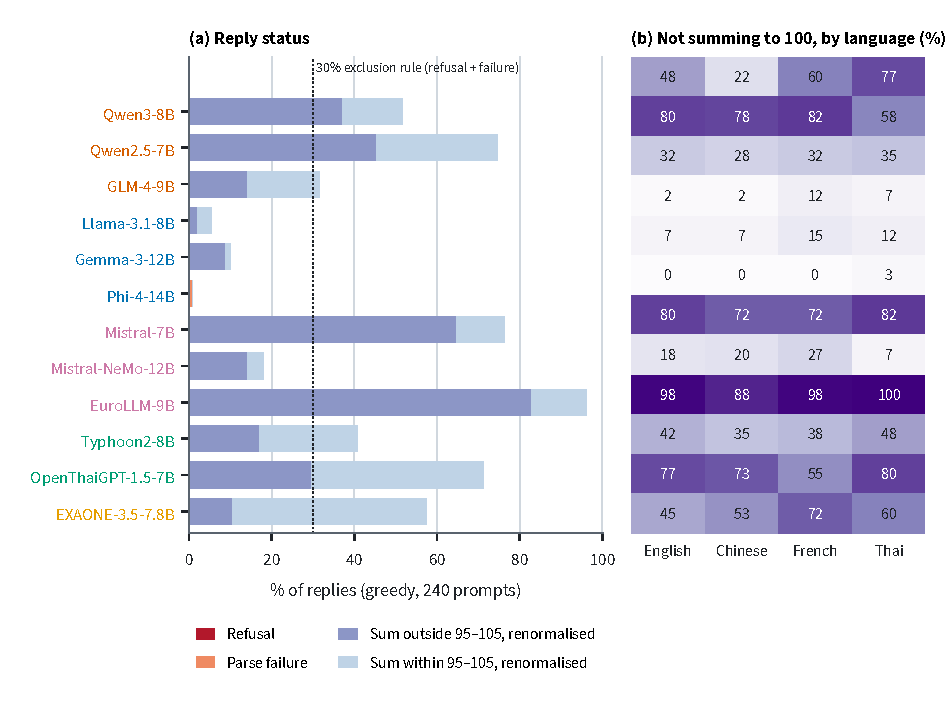
\includegraphics[width=\textwidth]{figures/fig5_refusal_parse_rates.pdf}
\caption{Reply status in the primary run. (a) Share of the 240 greedy replies per model by status: a reply gets one stricter retry if it is invalid or sums outside 95--105, and sums still outside 95--105 after the retry are renormalised (amendment A1). The dotted line is the 30\% exclusion rule for refusals plus parse failures. (b) Share of replies not summing to exactly 100, by prompt language.}
\label{fig:rates}
\end{figure}

\section{Reproduction and use of generative AI}\label{app:repro}

Code, prompts, all raw replies and the parsed panel are at \repo{}. \texttt{make all} rebuilds every number, table and figure from the cached replies in under a minute without a GPU, and \texttt{make paper} typesets this note; \texttt{make run} and \texttt{make robust} regenerate the replies with Ollama. The study was carried out with Claude (Anthropic), operated through the Claude Code agent, from the author's written brief, which fixed the question, hypotheses, design and decision rules. The agent wrote the pre-analysis plan and the code, ran the models, estimated the results and drafted this note; the author directed the work, reviewed the outputs and takes sole responsibility for the content. Every number in the text is generated from versioned result files.
